% $Id: firststart.tex 10592 2010-03-19 15:52:43Z alexandra $
% Local Variables:
% ispell-check-comments: nil
% Local IspellDict: american
% End:
% --------------------------------------------------------
% User documentation
% copyright by BREDEX GmbH 2004
% --------------------------------------------------------
%%\begin{bxdescription}

\index{ITE!Starting}
\index{Start!ITE}

\subsection{Windows Users}
\begin{enumerate}
\item Start the \ite{}  from the start menu:\\
\bxmenu{Start}{\gd{} or \jb{}}{\gd{} or \jb{}}.

\item You can also start the \ite{} using a command line argument.
\end{enumerate}

\subsection{Unix Users}
Enter the program name into the shell. 

\bxtipp{The \ite{} uses the current directory as its working directory on Linux systems.}

\subsection{Choosing a workspace}
\begin{enumerate}
\item When you start the \ite{}, a dialog appears asking you to choose a workspace (\bxfigref{WorkspaceChooser}).

\begin{figure}[h]
\begin{center}
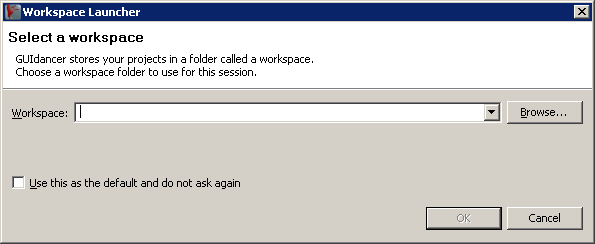
\includegraphics[width=0.7\textwidth]{Tasks/Start/PS/workspacechooser}
\caption{Workspace chooser}
\label{WorkspaceChooser}
\end{center}
\end{figure}

\bxtipp{The workspace is where your preferences are saved.}
\item Select the default workspace offered, or locate new one. 
\item You can choose to always select this workspace using the checkbox.
\bxtipp{You can see and change your workspace options in the preferences \bxpref{TasksPrefsWorkspace}.}
 \item Select \bxcaption{OK}.
 \end{enumerate}

\subsection{Restarting the \ite{}}
You can restart the \ite{} with the current workspace using:\\
\bxmenu{File}{Restart}{}

You can also restart the \ite{} with a new workspace by selecting:\\
\bxmenu{File}{Switch Workspace}{}





